\chapter{Search problems}



\section{Search strategies}
\begin{description}
    \item[Solution space] \marginnote{Solution space}
        Set of all the possible sequences of actions an agent may apply.
        Some of these lead to a solution.
    
    \item[Search algorithm] \marginnote{Search algorithm}
        Takes a problem as input and returns a sequence of actions that solves the problem (if exists).
\end{description}


\subsection{Search tree}
\begin{description}
    \item[Expansion] \marginnote{Expansion}
        Starting from a state, apply a successor function and generate a new state.

    \item[Search strategy] \marginnote{Search strategy}
        Choose which state to expand. 
        Usually is implemented using a fringe that decides which is the next node to expand.

    \item[Search tree] \marginnote{Search tree}
        Tree structure to represent the expansion of all states starting from a root 
        (i.e. the representation of the solution space).

        Nodes are states and branches are actions.
        A leaf can be a state to expand, a solution or a dead-end.
        \Cref{alg:search_tree_search} describes a generic tree search algorithm.

        \begin{figure}[h]
            \centering
            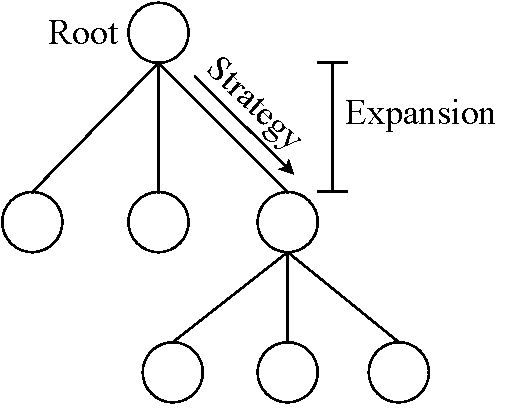
\includegraphics[width=0.25\textwidth]{img/_search_tree.pdf}
            \caption{Search tree}
        \end{figure}

        Each node contains:
        \begin{itemize}
            \item The state
            \item The parent node
            \item The action that led to this node
            \item The depth of the node
            \item The cost of the path from the root to this node
        \end{itemize}
\end{description}

\begin{algorithm}
\caption{Tree search} \label{alg:search_tree_search}
\begin{lstlisting}
def treeSearch(problem, fringe):
    fringe.push(problem.initial_state)
    # Get a node in the fringe and expand it if it is not a solution
    while fringe.notEmpty():
        node = fringe.pop()
        if problem.isGoal(node.state):
            return node.solution
        fringe.pushAll(expand(node, problem))
    return FAILURE

def expand(node, problem):
    successors = set()
    # List all neighboring nodes
    for action, result in problem.successor(node.state):
        s = new Node(
            parent=node, action=action, state=result, depth=node.dept+1,
            cost=node.cost + problem.pathCost(node, s, action)
        )
        successors.add(s)
    return successors
\end{lstlisting}
\end{algorithm}


\subsection{Strategies}
\begin{description}
    \item[Non-informed strategy] \marginnote{Non-informed strategy}
        Domain knowledge not available. Usually does an exhaustive search.

    \item[Informed strategy] \marginnote{Informed strategy}
        Use domain knowledge by using heuristics.
\end{description}


\subsection{Evaluation}
\begin{description}
    \item[Completeness] \marginnote{Completeness}
        if the strategy is guaranteed to find a solution (when exists).

    \item[Time complexity] \marginnote{Time complexity}
        time needed to complete the search.

    \item[Space complexity] \marginnote{Space complexity}
        memory needed to complete the search.

    \item[Optimality] \marginnote{Optimality}
        if the strategy finds the best solution (when more solutions are possible).
\end{description}



\section{Non-informed search}

\subsection{Breadth-first search (BFS)}
\marginnote{Breadth-first search}
Always expands the less deep node. The fringe is implemented as a queue (FIFO).

\begin{center}
    \def\arraystretch{1.2}
    \begin{tabular}{c | m{10cm}}
        \hline
        \textbf{Completeness} & Yes \\
        \hline
        \textbf{Optimality} & Only with uniform cost (i.e. all edges have same cost) \\
        \hline
        \textbf{\makecell{Time and space\\complexity}}
            & $O(b^d)$, where the solution depth is $d$ and the branching factor is $b$ (i.e. each non-leaf node has $b$ children) \\
        \hline
    \end{tabular}
\end{center}

The exponential space complexity makes BFS impractical for large problems.

\begin{figure}[h]
    \centering
    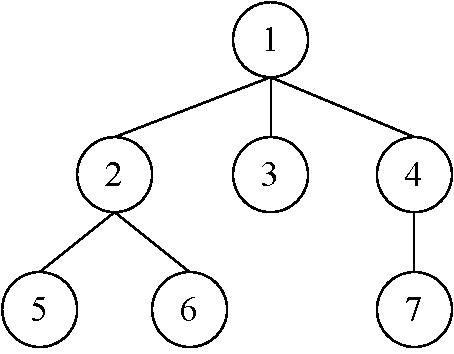
\includegraphics[width=0.30\textwidth]{img/_bfs.pdf}
    \caption{BFS visit order}
\end{figure}


\subsection{Uniform-cost search}
\marginnote{Uniform-cost search}
Same as BFS, but always expands the node with the lowest cumulative cost. 

\begin{center}
    \def\arraystretch{1.2}
    \begin{tabular}{c | m{10cm}}
        \hline
        \textbf{Completeness} & Yes \\
        \hline
        \textbf{Optimality} & Yes \\
        \hline
        \textbf{\makecell{Time and space\\complexity}}
            & $O(b^d)$, with solution depth $d$ and branching factor $b$ \\
        \hline
    \end{tabular}
\end{center}

\begin{figure}[h]
    \centering
    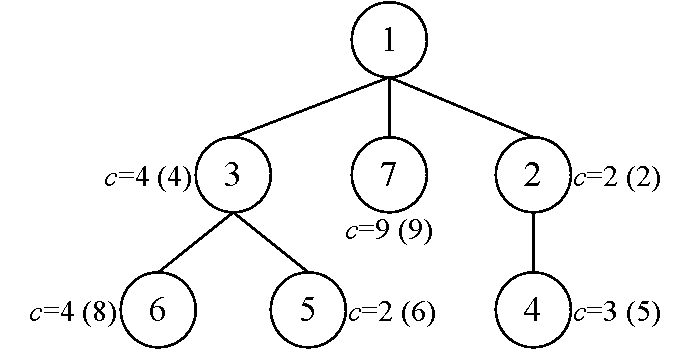
\includegraphics[width=0.50\textwidth]{img/_ucs.pdf}
    \caption{Uniform-cost search visit order. $(n)$ is the cumulative cost}
\end{figure}


\subsection{Depth-first search (DFS)}
\marginnote{Depth-first search}
Always expands the deepest node. The fringe is implemented as a stack (LIFO).

\begin{center}
    \def\arraystretch{1.2}
    \begin{tabular}{c | m{10cm}}
        \hline
        \textbf{Completeness} & No (loops) \\
        \hline
        \textbf{Optimality} & No \\
        \hline
        \textbf{Time complexity}
            & $O(b^m)$, with maximum depth $m$ and branching factor $b$ \\
        \hline
        \textbf{Space complexity}
            & $O(b \cdot m)$, with maximum depth $m$ and branching factor $b$ \\
        \hline
    \end{tabular}
\end{center}

\begin{figure}[h]
    \centering
    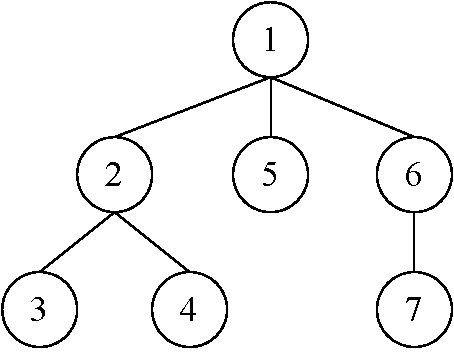
\includegraphics[width=0.30\textwidth]{img/_dfs.pdf}
    \caption{DFS visit order}
\end{figure}


\subsection{Depth-limited search}
\marginnote{Depth-limited search}
Same as DFS, but introduces a maximum depth.
A node at the maximum depth will not be explored further.

This allows to avoid infinite branches (i.e. loops).



\subsection{Iterative deepening}
\marginnote{Iterative deepening}
Runs a depth-limited search by trying all possible depth limits.
It is important to note that each iteration is executed from scratch (i.e. a new execution of depth-limited search).

\begin{algorithm}
\caption{Iterative deepening}
\begin{lstlisting}
def iterativeDeepening(G):
    for c in range(G.max_depth):
        sol = depthLimitedSearch(G, c)
        if sol is not FAILURE:
            return sol
    return FAILURE
\end{lstlisting}
\end{algorithm}

Both advantages of DFS and BFS are combined.

\begin{center}
    \def\arraystretch{1.2}
    \begin{tabular}{c | m{10cm}}
        \hline
        \textbf{Completeness} & Yes \\
        \hline
        \textbf{Optimality} & Only with uniform cost \\
        \hline
        \textbf{Time complexity}
            & $O(b^d)$, with solution depth $d$ and branching factor $b$ \\
        \hline
        \textbf{Space complexity}
            & $O(b \cdot d)$, with solution depth $d$ and branching factor $b$ \\
        \hline
    \end{tabular}
\end{center}



\section{Informed search}
\marginnote{Informed search}
Informed search uses evaluation functions (heuristics) to reduce the search space and
estimate the effort needed to reach the final goal.


\subsection{Best-first search}
\marginnote{Best-first seacrh}
Uses heuristics to compute the desirability of the nodes (i.e. how close they are to the goal).
The fringe is ordered according the estimated scores.


\begin{description}
    \item[Greedy search / Hill climbing] 
        \marginnote{Greedy search / Hill climbing}
        The heuristic only evaluates nodes individually and does not consider the path to the root
        (i.e. expands the node that currently seems closer to the goal).
        \begin{center}
            \def\arraystretch{1.2}
            \begin{tabular}{c | m{9cm}}
                \hline
                \textbf{Completeness} & No (loops) \\
                \hline
                \textbf{Optimality} & No \\
                \hline
                \textbf{\makecell{Time and space\\complexity}}
                & $O(b^d)$, with solution depth $d$ and branching factor $b$ \\
            \hline
            \end{tabular}
        \end{center}
        % The complexity can be reduced depending on the heuristic.

        \begin{figure}[ht]
            \centering
            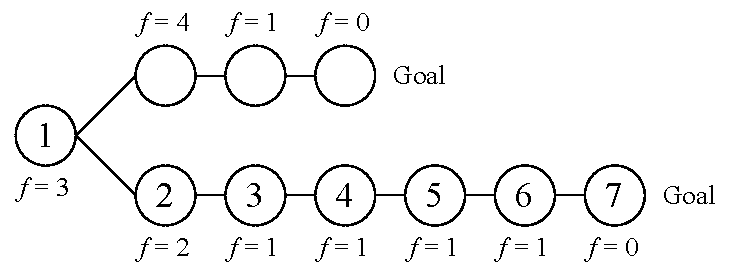
\includegraphics[width=0.65\textwidth]{img/_greedy_best_first_example.pdf}
            \caption{Hill climbing visit order}
        \end{figure}

    \item[A$^\textbf{*}$]
        \marginnote{A$^*$}
        The heuristic also considers the cumulative cost needed to reach a node from the root.
        The score associated to a node $n$ is:
        \[ f(n) = g(n) + h'(n) \]
        where $g$ is the depth of the node and $h'$ is the heuristic that computes the distance to the goal.

        \begin{description}
            \item[Optimistic/Feasible heuristic]
            \marginnote{Optimistic/Feasible heuristic}
            Given $t(n)$ that computes the true distance of a node $n$ to the goal.
            An heuristic $h'(n)$ is optimistic (i.e. feasible) if:
            \[ h'(n) \leq t(n) \]
            In other words, $h'$ is optimistic if it always underestimates the distance to the goal.
        \end{description}

        \begin{theorem}
            If the heuristic used by A${^*}$ is optimistic $\Rightarrow$ A${^*}$ is optimal
        \end{theorem}
        \begin{proof}
            Consider a scenario where the queue contains:
            \begin{itemize}
                \item A node $n$ whose child is the optimal solution
                \item A sub-optimal solution $G_2$
            \end{itemize}
            \begin{center}
                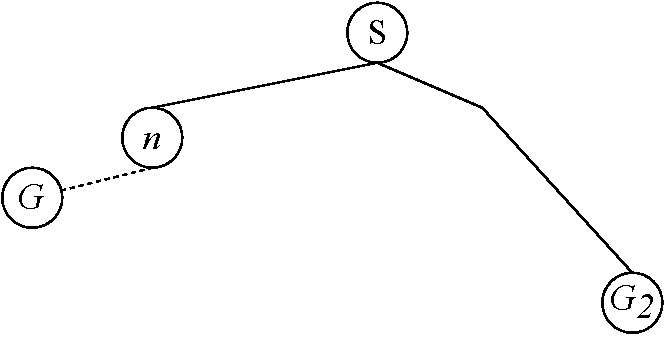
\includegraphics[width=0.5\textwidth]{img/_a_start_optimality.pdf}
            \end{center}
            We want to prove that A$^*$ will always expand $n$.

            Given an optimistic heuristic $f(n) = g(n) + h'(n)$ and
            the true distance of a node $n$ to the goal $t(n)$,
            we have that:
            \[
                \begin{split}
                    f(G_2) &= g(G_2) + h'(G_2) = g(G_2) \text{, as } G_2 \text{ is a solution: } h'(G_2)=0 \\
                    f(G) &= g(G) + h'(G) = g(G) \text{, as } G \text{ is a solution: } h'(G)=0
                \end{split}
            \]
            Moreover, $g(G_2) > g(G)$ as $G_2$ is suboptimal.
            Therefore, $\bm{f(G_2) > f(G)}$.

            Furthermore, as $h'$ is feasible, we have that:
            \[
                \begin{split}
                    h'(n) \leq t(n) &\iff g(n) + h'(n) \leq g(n) + t(n) = g(G)=f(G) \\
                        &\iff \bm{f(n) \leq f(G)}
                \end{split}  
            \]
            In the end, we have that $f(G_2) > f(G) \geq f(n)$.
            So we can conclude that A$^*$ will never expand $G_2$ as:
            \[ f(G_2) > f(n) \] 
        \end{proof}

        \begin{center}
            \def\arraystretch{1.2}
            \begin{tabular}{c | m{9cm}}
                \hline
                \textbf{Completeness} & Yes \\
                \hline
                \textbf{Optimality} & Only if the heuristic is optimistic \\
                \hline
                \textbf{\makecell{Time and space\\complexity}}
                & $O(b^d)$, with solution depth $d$ and branching factor $b$ \\
            \hline
            \end{tabular}
        \end{center}

        In generally, it is better to use heuristics with large values (i.e. heuristics that don't underestimate too much).

        \begin{figure}[ht]
            \centering
            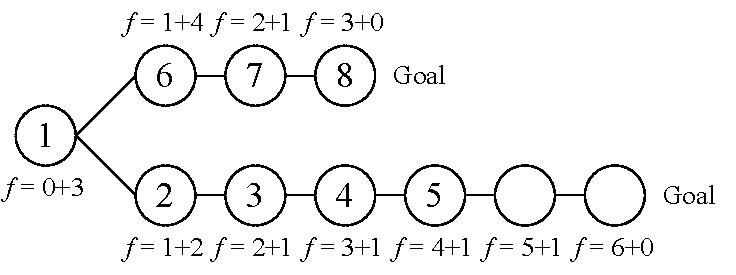
\includegraphics[width=0.65\textwidth]{img/_a_start_example.pdf}
            \caption{A$^*$ visit order}
        \end{figure}
\end{description}


\section{Graph search}
\marginnote{Graph search}
Differently from a tree search, searching in a graph requires to keep track of the explored nodes.
\begin{algorithm}
    \caption{Graph search} \label{alg:search_graph_search}
    \begin{lstlisting}
    def graphSearch(problem, fringe):
        closed = set()
        fringe.push(problem.initial_state)
        # Get a node in the fringe and 
        # expand it if it is not a solution and is not closed
        while fringe.notEmpty():
            node = fringe.pop()
            if problem.isGoal(node.state):
                return node.solution
            if node.state not in closed:
                closed.add(node.state)
                fringe.pushAll(expand(node, problem))
        return FAILURE
    \end{lstlisting}
\end{algorithm}


\subsection{A$^\textbf{*}$ with graphs}
\marginnote{A$^*$ with graphs}
The algorithm keeps track of closed and open nodes.
The heuristic $g(n)$ evaluates the minimum distance from the root to the node $n$.

\begin{description}
    \item[Consistent heuristic (monotone)] \marginnote{Consistent heuristic (monotone)}
    An heuristic is consistent if for each $n$, for any successor $n'$ of $n$ (i.e. nodes reachable from $n$ by making an action)
    holds that:
    \[ 
        \begin{cases}
            h(n) = 0 & \text{if the corresponding status is the goal} \\
            h(n) \leq c(n, a, n') + h(n') & \text{otherwise}
        \end{cases}
    \]
    where $c(n, a, n')$ is the cost to reach $n'$ from $n$ by taking the action $a$.

    In other words, $f$ never decreases along a path.
    In fact:\\
    \begin{minipage}{.48\linewidth}
        \[  
            \begin{split}
                f(n') &= g(n') + h(n') \\
                    &= g(n) + c(n, a, n') + h(n') \\
                    &\geq g(n) + h(n) \\
                    &= f(n)
            \end{split}
        \]
    \end{minipage}
    \begin{minipage}{.48\linewidth}
        \centering
        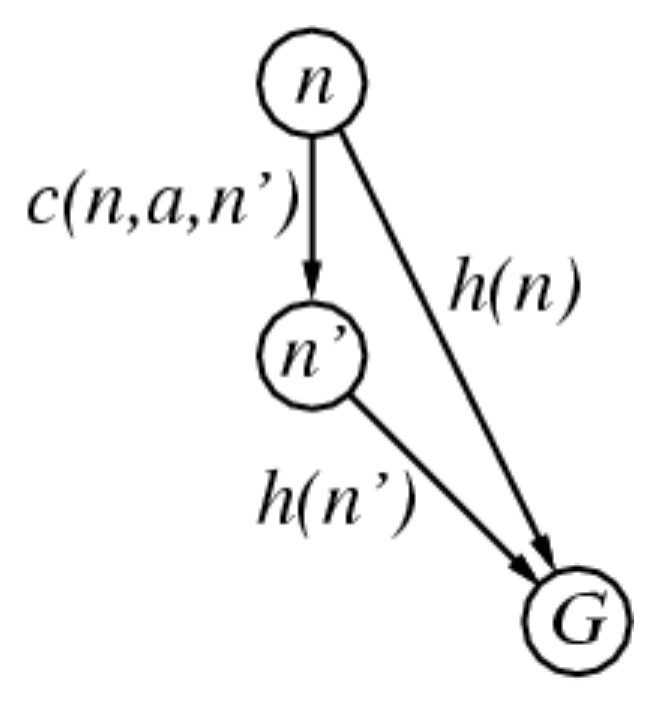
\includegraphics[width=0.3\textwidth]{img/monotone_heuristic.png}
    \end{minipage}


    \begin{theorem}
        If $h$ is a consistent heuristic, A$^*$ on graphs is optimal.
    \end{theorem}
\end{description}
